\documentclass[xetex,mathserif,serif]{beamer}
\usepackage{polyglossia}
\setdefaultlanguage[babelshorthands=true]{russian}
\usepackage{minted}
\usepackage{tabu}

\useoutertheme{infolines}

\usepackage{fontspec}
\setmainfont{FreeSans}
\newfontfamily{\russianfonttt}{FreeSans}

\setbeamertemplate{blocks}[rounded][shadow=false]
\setbeamercolor*{block title example}{fg=green!50!black,bg=green!20}
\setbeamercolor*{block body example}{fg=black,bg=green!10}

\setbeamercolor*{block title alerted}{fg=red!50!black,bg=red!20}
\setbeamercolor*{block body alerted}{fg=black,bg=red!10}

\tabulinesep=0.7mm

\title{Практика}
\author[Юрий Литвинов]{Юрий Литвинов \newline \textcolor{gray}{\small\texttt{yurii.litvinov@gmail.com}}}

\date{23.03.2017г}

\begin{document}
	
	\frame{\titlepage}
	
	\section{Слоистая архитектура для VCS}

	\begin{frame}
		\frametitle{Архитектура VCS, уровень пользователя}
		\begin{center}
			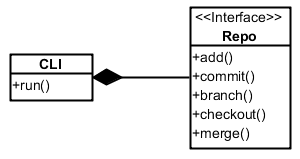
\includegraphics[width=0.35\textwidth]{vcsInterfaceLevel.png}
		\end{center}
	\end{frame}

	\begin{frame}
		\frametitle{Архитектура VCS, команды}
		\begin{center}
			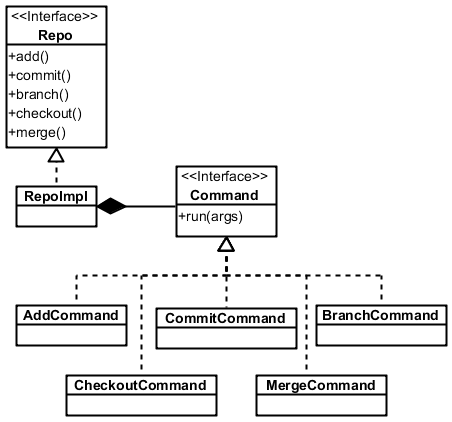
\includegraphics[width=0.55\textwidth]{vcsCommandsHierarchy.png}
		\end{center}
	\end{frame}

	\begin{frame}
		\frametitle{Архитектура VCS, уровень бизнес-логики}
		\begin{center}
			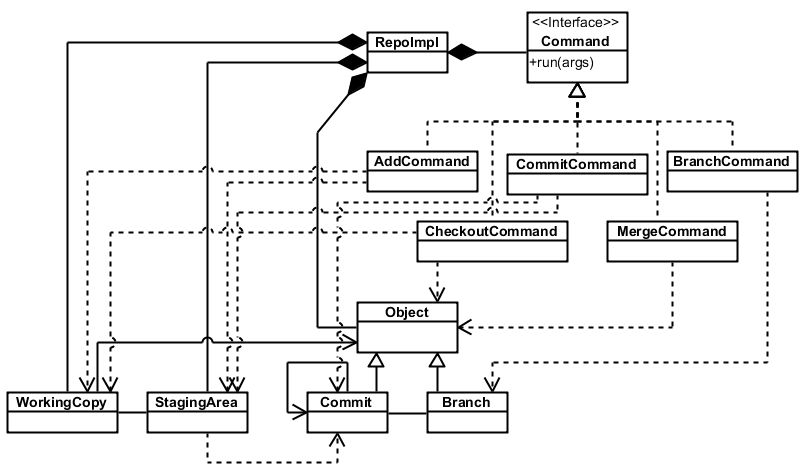
\includegraphics[width=0.9\textwidth]{vcsDomainModel.png}
		\end{center}
	\end{frame}

	\begin{frame}
		\frametitle{Архитектура VCS, уровень данных}
		\begin{center}
			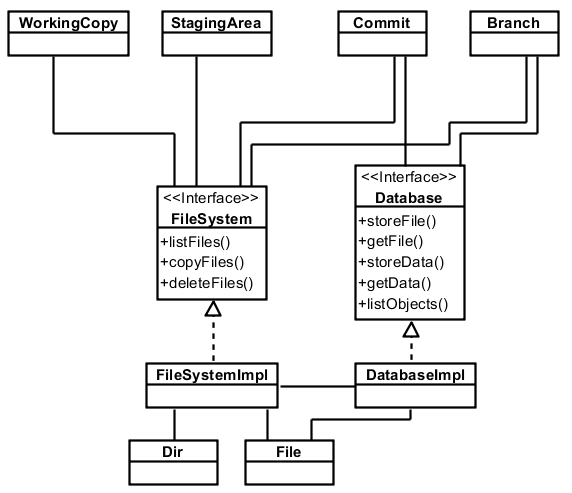
\includegraphics[width=0.7\textwidth]{vcsDataLayer.png}
		\end{center}
	\end{frame}

	\begin{frame}
		\frametitle{Архитектура VCS, итог}
		\begin{center}
			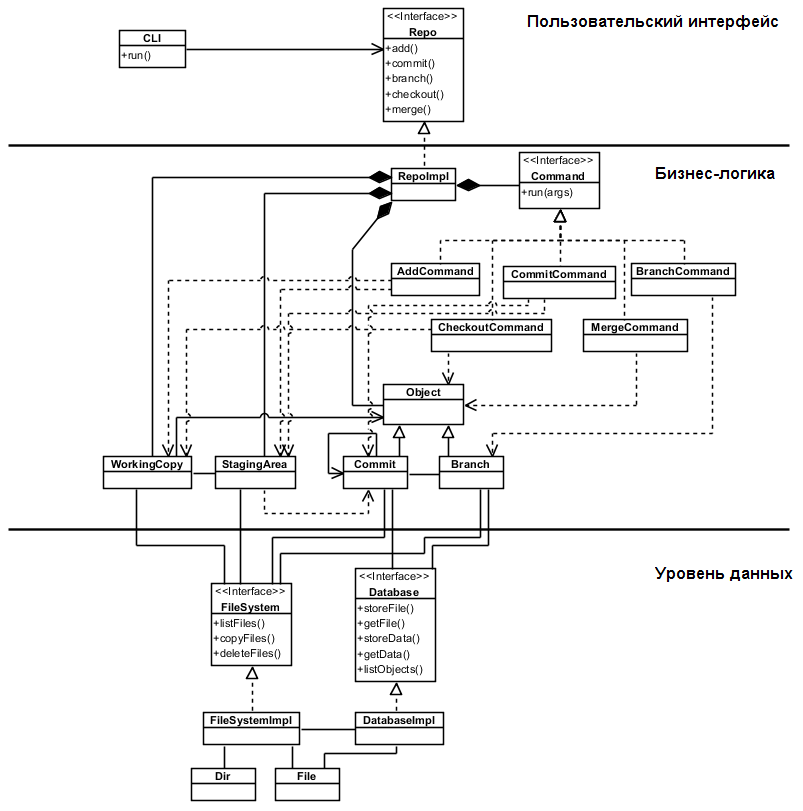
\includegraphics[width=0.63\textwidth]{vcsOverallArchitecture.png}
		\end{center}
	\end{frame}

	\section{Задача на пару}

	\begin{frame}
		\frametitle{Задача, CountdownLatch}
		\framesubtitle{Репетиция контрольной}
		Реализовать свой собственный CountdownLatch (но хитрый):
		\begin{itemize}
			\item Конструктор, принимающий число (счётчик) в качестве аргумента
			\item Метод \mintinline{java}|await()|, который блокирует вызвавший его поток, пока счётчик не станет равным нулю
			\item Метод \mintinline{java}|countDown()|, который уменьшает счётчик на 1 и запускает все потоки, заблокированные на await, если счётчик достиг 0
			\begin{itemize}
				\item Если счётчик и так 0, \mintinline{java}|countDown()| блокирует поток до тех пор, пока счётчик не станет положительным, потом уменьшает его
			\end{itemize}
			\item Метод \mintinline{java}|countUp()|, который увеличивает счётчик на 1 и запускает потоки, заблокированные на \mintinline{java}|countDown()|, если такие есть
			\item Нельзя использовать synchronized
			\begin{itemize}
				\item Можно Lock/Condition
			\end{itemize}
		\end{itemize}
	\end{frame}

\end{document}
